\documentclass{../codeproblem}

\begin{document}
\title{Planning Operations}
\begin{flavor}
  With our trusty zip-lines, there's no way the Evil Empire of Evil can beat us!
\end{flavor}



In order to infiltrate the EEE's facilities, our elite agents use zip-lines to travel from building to building. However, this means that each leg of our journey must be in a straight line. In order to achieve maximum stealth, we must carefully plan our route to include as few course changes as possible.

Given an 8x8 grid, write a program to find the route from the bottom left corner (0, 0) to the top right corner (7, 7) with the fewest number of course changes. Only the minimum number of course changes possible is required, not the actual path (as their may be several ``best'' solutions).

\begin{figure}[h!]
  \centering
  
\includegraphics[width=2.0in]{pics/emptygrid}
\end{figure}

Input will be given as a series of coordinates defining tiles that are impassable. These coordinates will be given as two space-separated integers ranging from 0 to 7. You can assume that no more than 20 tiles will be impassable and that there will always be a valid route from (0, 0) to (7, 7).

Output should be the minimum number of turns required to reach (7, 7) from (0, 0), expressed as an integer.

\section*{Examples}

Examples below include the grid represented by the given tiles, as well as at least one valid shortest path.

\begin{minipage}{.5\linewidth}
\begin{example}
0
|\textbf{1}\end{example}
\end{minipage}
\begin{minipage}{.5\linewidth}
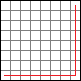
\includegraphics[width=.5\linewidth]{pics/simplest}
\end{minipage}

\begin{minipage}{.5\linewidth}
\begin{example}
0 3
0 5
2 4
3 2
3 3
4 1
4 5
4 6
5 2
5 7
6 0
6 5
7 2
0
|\textbf{1}\end{example}
\end{minipage}
\begin{minipage}{.5\linewidth}
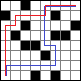
\includegraphics[width=.6\linewidth]{pics/example}
\end{minipage}


\end{document}
